\documentclass[letterpaper,12pt]{article}
\usepackage{tabularx} % extra features for tabular environment
\usepackage{amsmath}  % improve math presentation
\usepackage{graphicx} % takes care of graphic including machinery
\graphicspath{ {./figures/} }
\usepackage[margin=1in,letterpaper]{geometry} % decreases margins
\usepackage{cite} % takes care of citations
\usepackage[final]{hyperref} % adds hyper links inside the generated pdf file
\hypersetup{
	colorlinks=true,       % false: boxed links; true: colored links
	linkcolor=blue,        % color of internal links
	citecolor=blue,        % color of links to bibliography
	filecolor=magenta,     % color of file links
	urlcolor=blue         
}
%++++++++++++++++++++++++++++++++++++++++


\begin{document}

\title{Experiment 2 \protect\\Signal Generators and Oscilloscopes}
\author{Ahmet Akman \protect\\ Assistant : Etki Açılan}
\date{\today}
\maketitle

%\begin{abstract}
%abstract
%\end{abstract}


\section{Introduction} 
In this experiment, as students we are expected to experiment how to use the function generators and oscilloscopes by completing the steps described in second experiment laboratory manual. Throughtout these steps, the monitoring properties of the oscilloscope , different output forms of the signal generator observed via connecting the instruments directly each other and to the circuit. The results of the steps noted and plotted for the further comments.
\section{Experimental Results}
In this section the results of the Experiment 2 are discussed.
\subsection{Step 1}
In this step only the oscilloscope instrument used. The probes of the "Channel 1" is connected to the "Prob Comp" terminals which supplies square waveform. After adjusting the monitor scale using "AutoScale" button, peak to peak value is observed from the grids of the monitor. Peak to peak voltage is measured as "2.40 Volts". When "Vertical Division Control" rotary button adjusted to different positions the voltage values of which the grids represents differs. When "Vertical Position Control" rotary button adjusted to diferent positions the signal moves in vertical position without changing its from. The "Horizontal Division Control" rotary button is used to scale the time steps for the active signal. The "Horizontal Position Control" is used to regulate the delay of the signal display. By observing the channel axis control buttons' functions the step 1 is completed.
\subsection{Step 2}
In Step 2, the oscilloscope and probing setup is conserved as described in Step 1. After making sure the channel 1 is activated, the substeps of a. and b. followed.
\subsubsection{a.}
The coupling method is adjusted using the on-screen menu. The difference between "DC" and "AC" coupling method is observed from the square waveform. As given in the figure "AC" coupling method ignores the DC component of the signal. Unlike "DC" setting "AC" setting is especially used for the change on the waveform.
\begin{figure}[h]
	\caption{AC Coupling Plot}
	\centering
	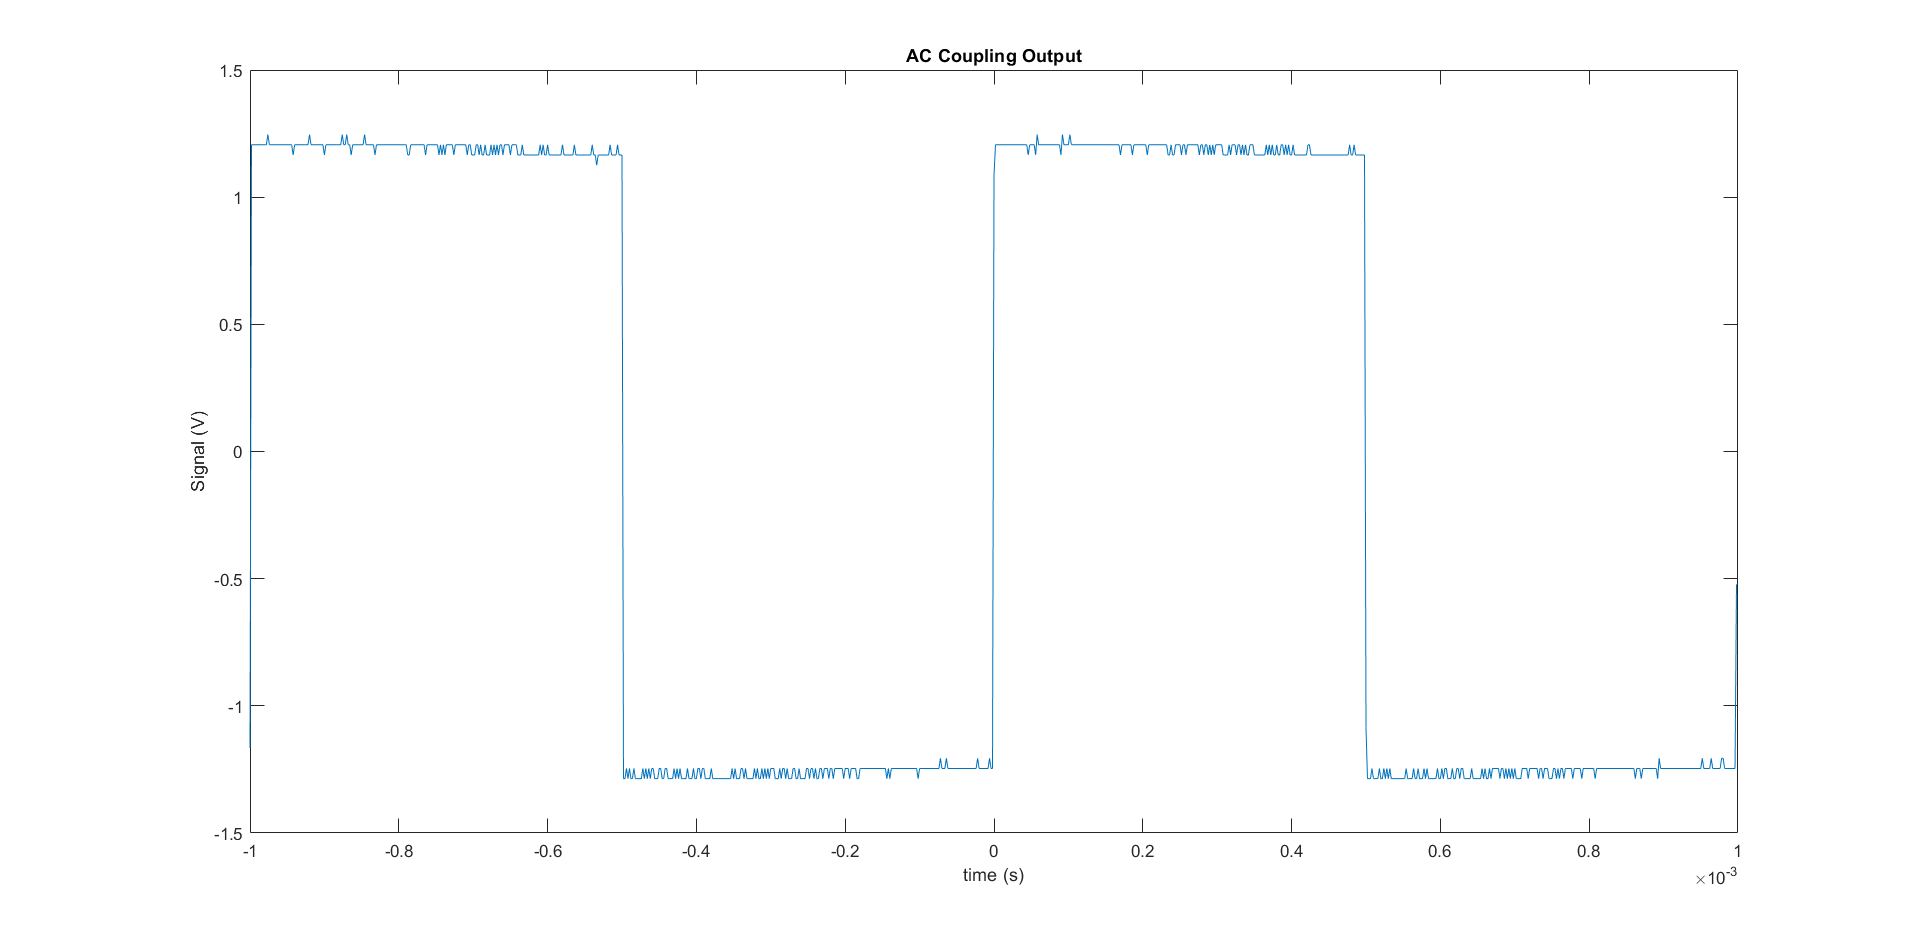
\includegraphics[width=1\textwidth]{2a.png}
\end{figure}

\subsubsection{b.}
The coupling method is adjusted using the on-screen menu and the DC coupled waveform is inverted. The plot of DC coupled signal is shown in the Figure 2.

\begin{figure}[h]
	\caption{DC Coupling Plot}
	\centering
	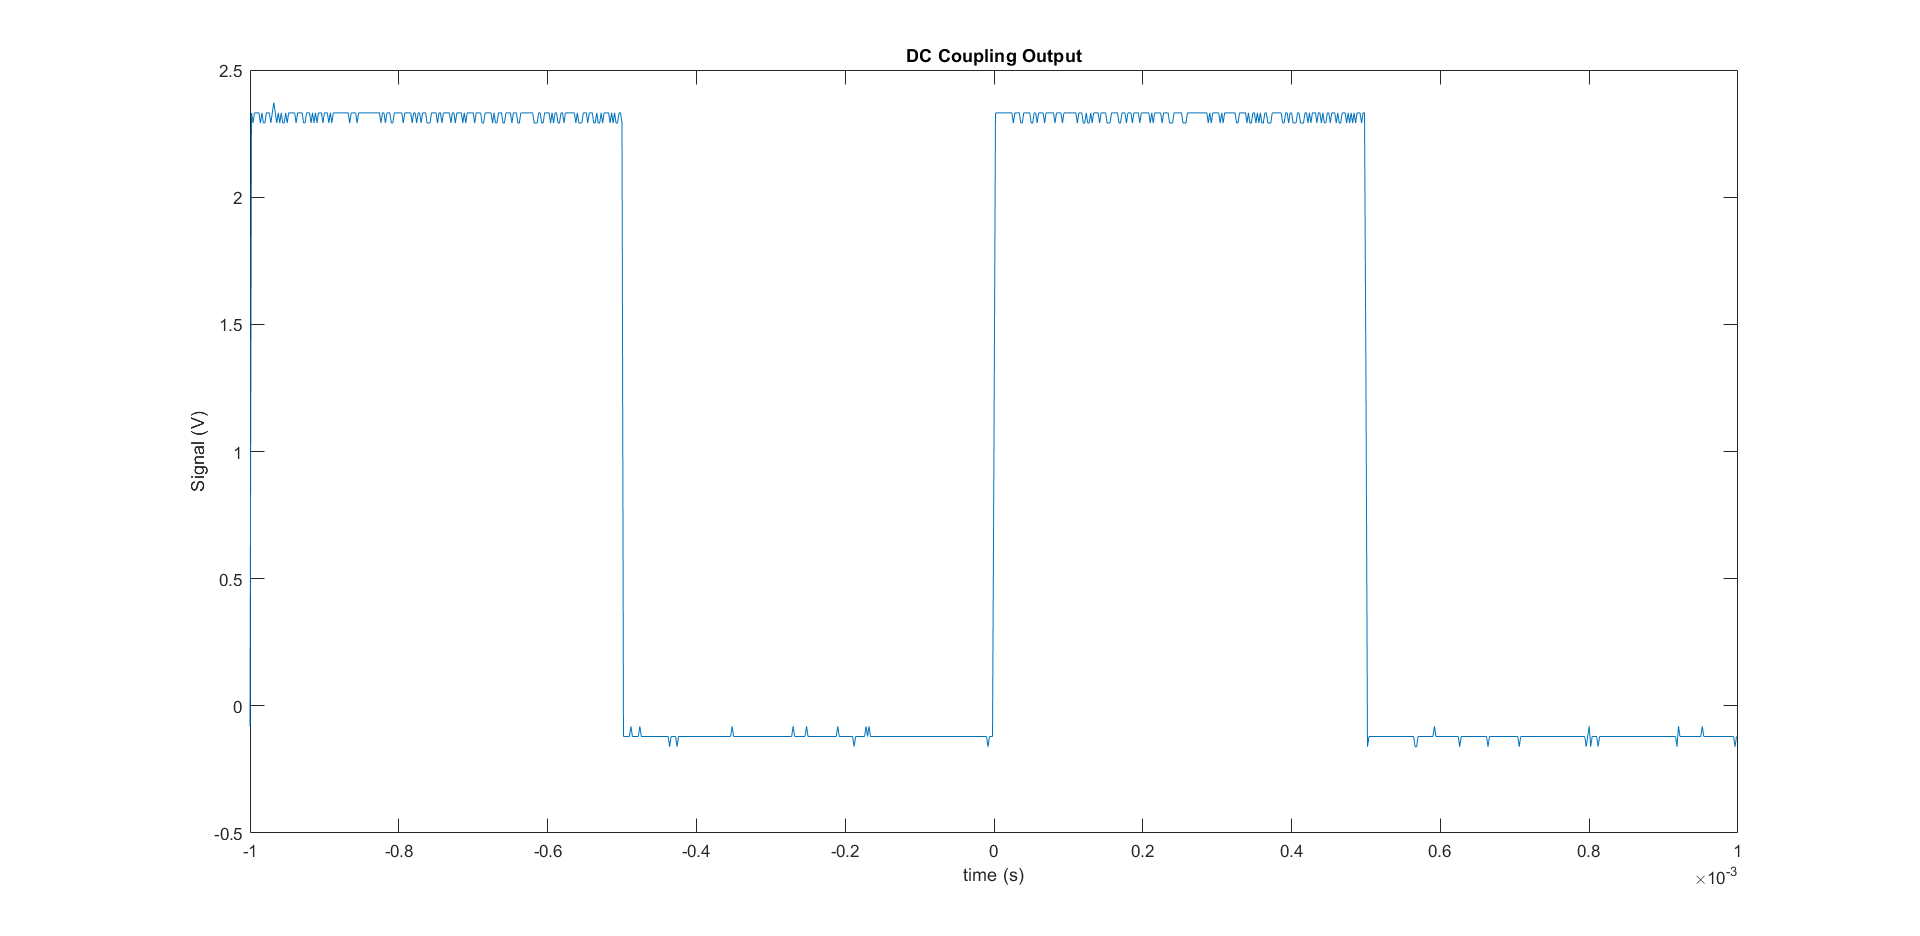
\includegraphics[width=1\textwidth]{2b1.png}
\end{figure}
The inverted form of the DC coupled signal is observed. The plot of the inverted form is shown in the Figure 3.

\begin{figure}[h]
	\caption{DC Coupling Inverted Plot}
	\centering
	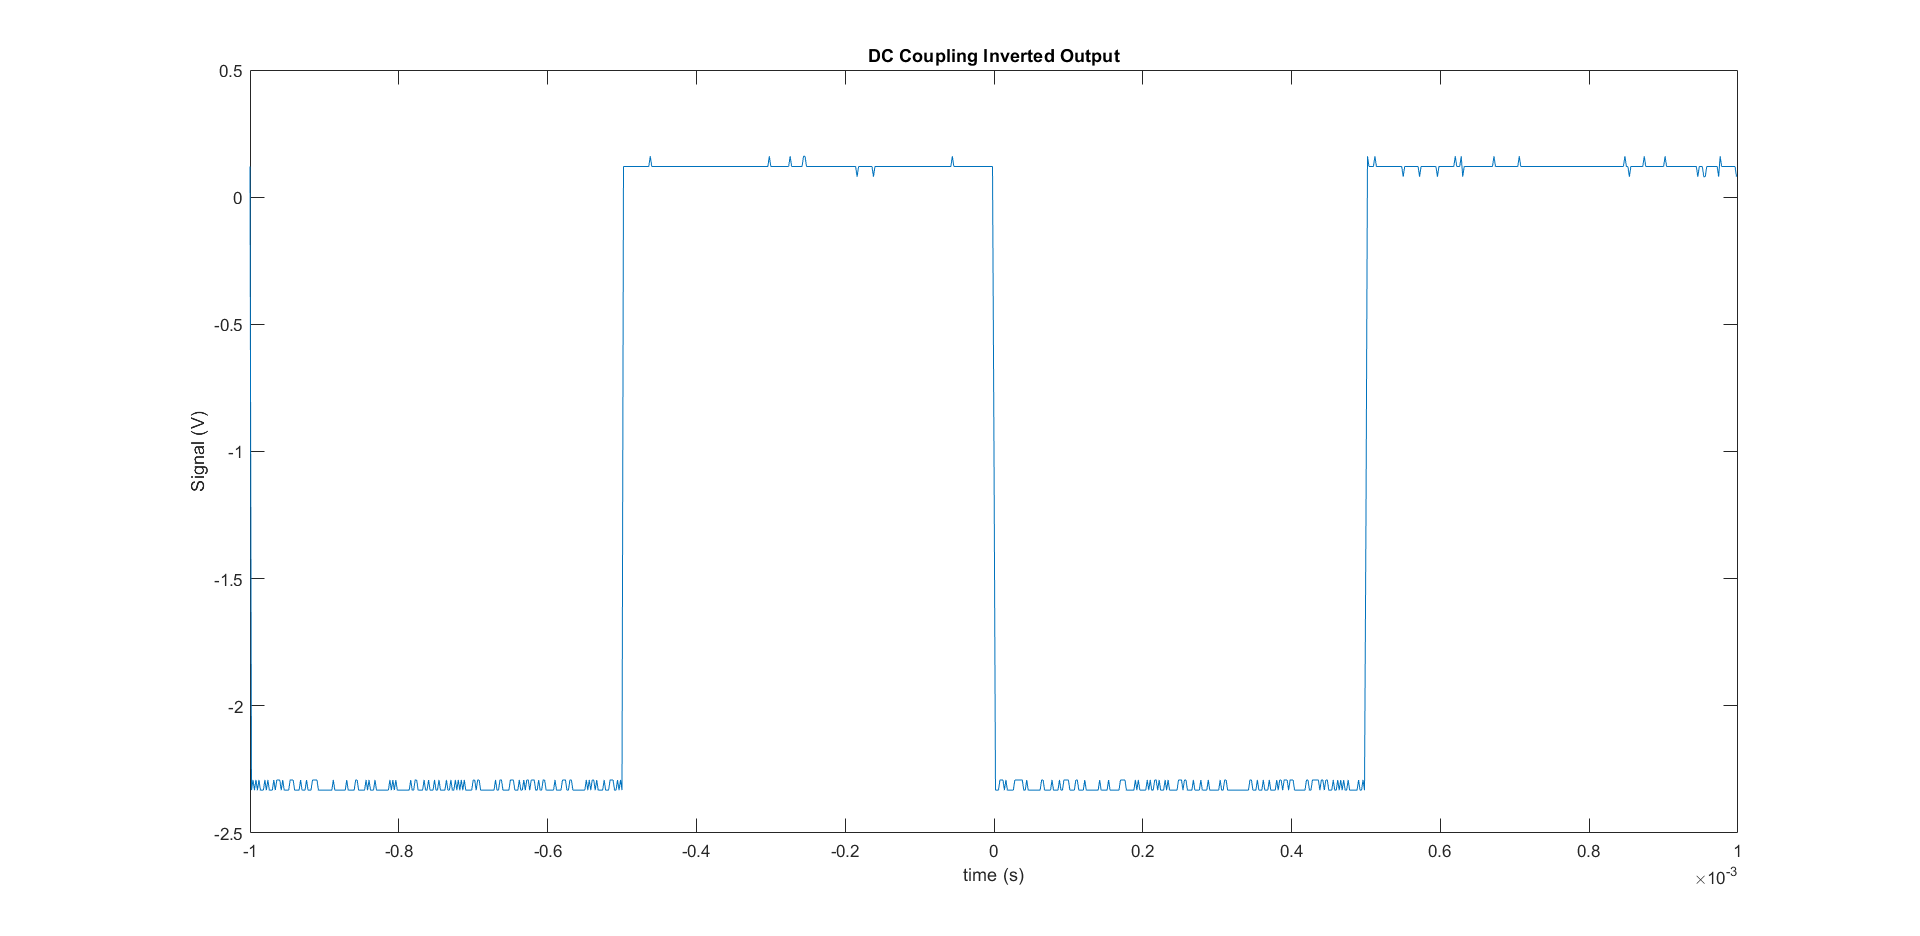
\includegraphics[width=1\textwidth]{2b2.png}
\end{figure}
When the signal is inverted, the inverse of the measured values become displayed. So that the values are multplied with -1. 

\subsection{Step 3}
In this step procedures that are followed during the first and second steps are repeated for the "Channel 2". The figures displayed are verified to be same for the second channel. Although the substeps are significantly same, there are seperated button sets on the oscilloscope panel.
\subsection{Step 4}
In this step only the oscilloscope instrument used. The probes of the "Channel 1" is connected to the "Prob Comp" terminals which generates square waveform.
\subsubsection{a.}
Using the "Cursors" button and "Cursors Knob" cursors of Y1 and Y2 adjusted while source "1" is selected.
\subsubsection{b.}
By adjusting Y1 and Y2 cursors to the peaks of the waveform, peak to peak voltage is measured as "2.45 Volts".
\subsubsection{c.}
By setting the "Cursors Knob" for X1 and X2 cursors verticallly, period is measured as "500 \(\mu\)s" then the frequency is calculated from the equation "  \( \frac{1}{period} \) " as "1.00 kHz".

\subsection{Step 5}
In Step 5, the oscilloscope and probing setup is conserved as described in Step 4. While the relevant channel is selected, measure button is pressed.
\subsubsection{a.}
Using type soft  button on the display panel measurement type is selected "Peak-Peak" then the measurement taken as "2.59 Volts"
\subsubsection{b.}
Using button indicating type on the display panel measurement type is selected "Period" then the measurement obtained as "998.84 \(\mu\)s"
\subsection{Step 6}
In this step, oscillator and function waveform generator instruments are used. The function waveform generator is set sine waveform 2 kHz on "High Z" option. The circuit constructed on the breadboard can be seen from the Figure 4. The inputs of the oscilloscope connected CH1 and CH2 terminals accordingly.
\begin{figure}[h]
	\caption{The circuit diagram for the Step 6}
	\centering
	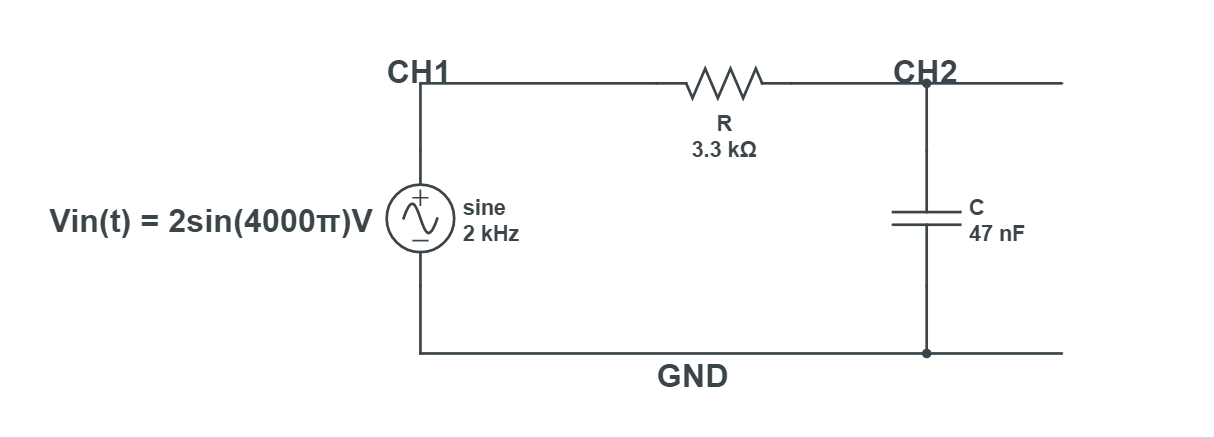
\includegraphics[width=1\textwidth]{6circuit.png}
\end{figure}

\subsubsection{a.}
In Figure 5, \( V_{in}\) (t) at Channel 1 ,\( V_0 \) (t) at Channel 2 is shown. The phase difference between the signals is measured as "65.\(\overline{45}\)  degrees" using the DSO cursors. The horizontal mode is set as time for the Figure 5.

\begin{figure}[h]
	\caption{\( V_{in}\) (t) at Channel 1 ,\( V_0 \) (t) at Channel 2  }
	\centering
	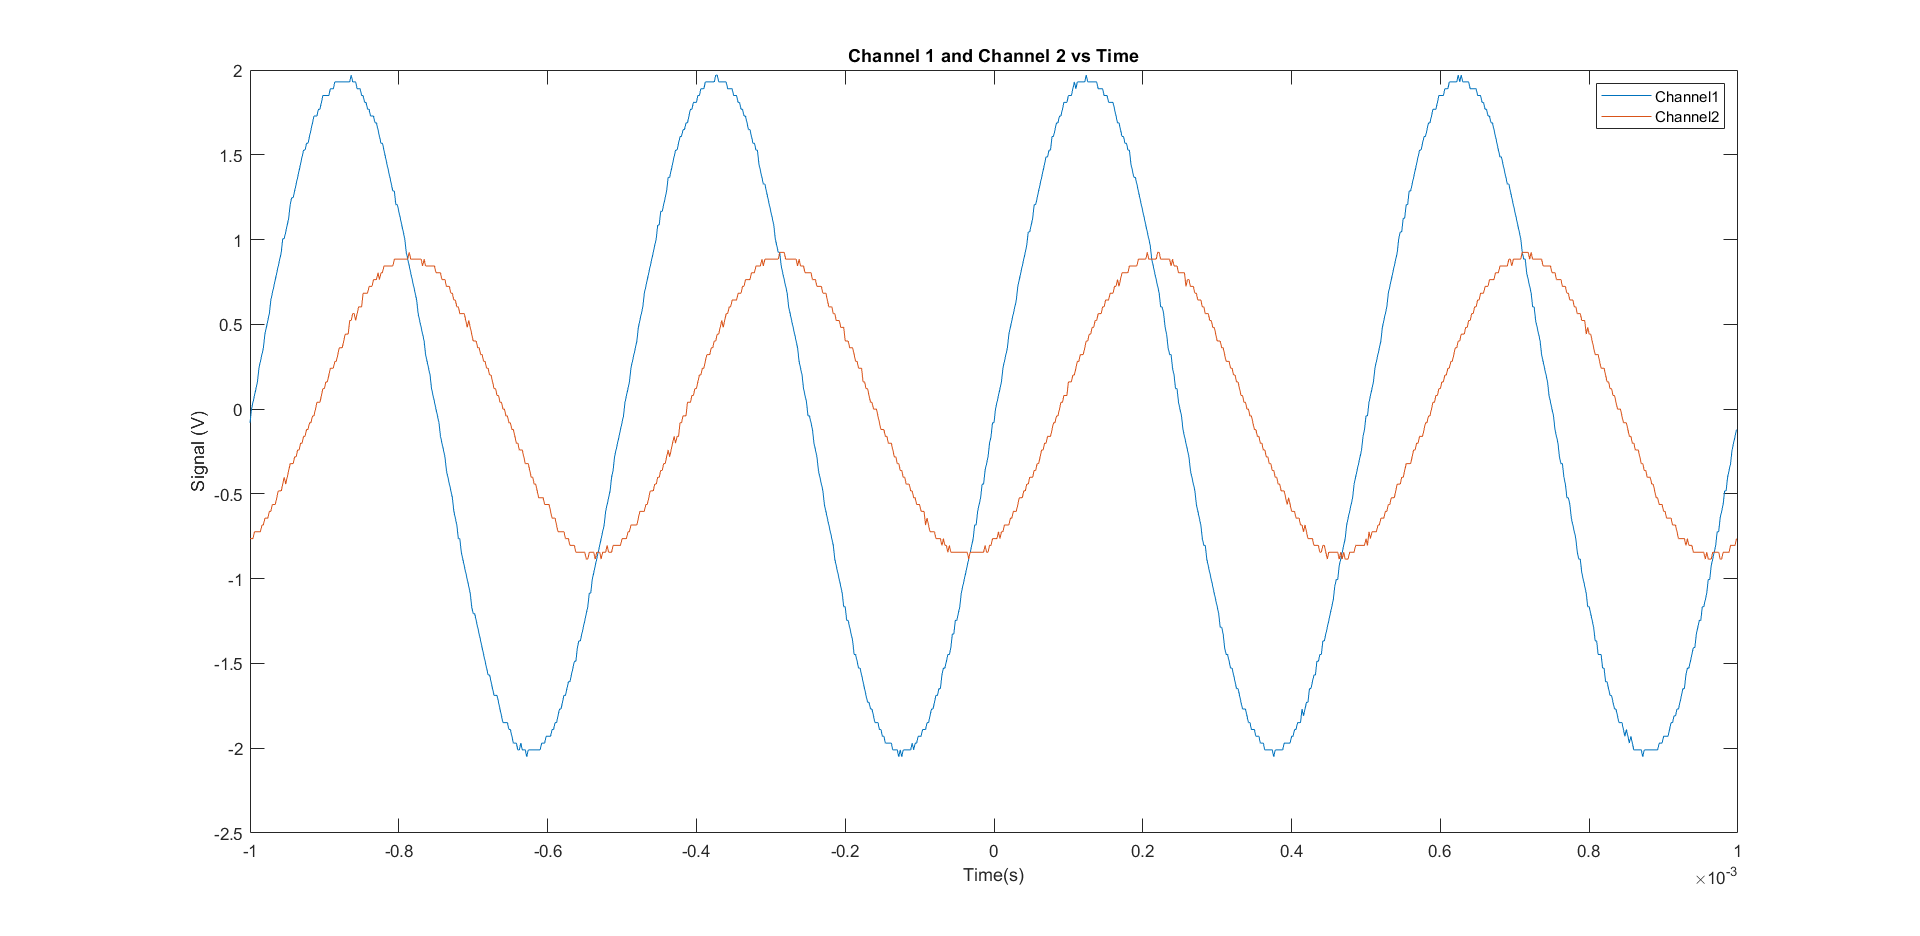
\includegraphics[width=1\textwidth]{6a.png}
\end{figure}

\subsubsection{b.}
In Figure 6, \( V_{in}\) at Channel 1 ,\( V_0 \) at Channel 2 is shown. The phase difference between the signals is measured as "63.78211805 degrees" using the DSO cursors' Y1 and Y2 . The difference between Y axis interception points denoted as A and  difference between the boundary points are denoted as B. Then using the \(arcsin({A}/{B})\) formula the phase difference is determined. The XY mode is set as time option for the Figure 6.
\begin{figure}[h]
	\caption{\( V_{in}\) (t) at X axis \( V_0 \) (t) at Y axis  }
	\centering
	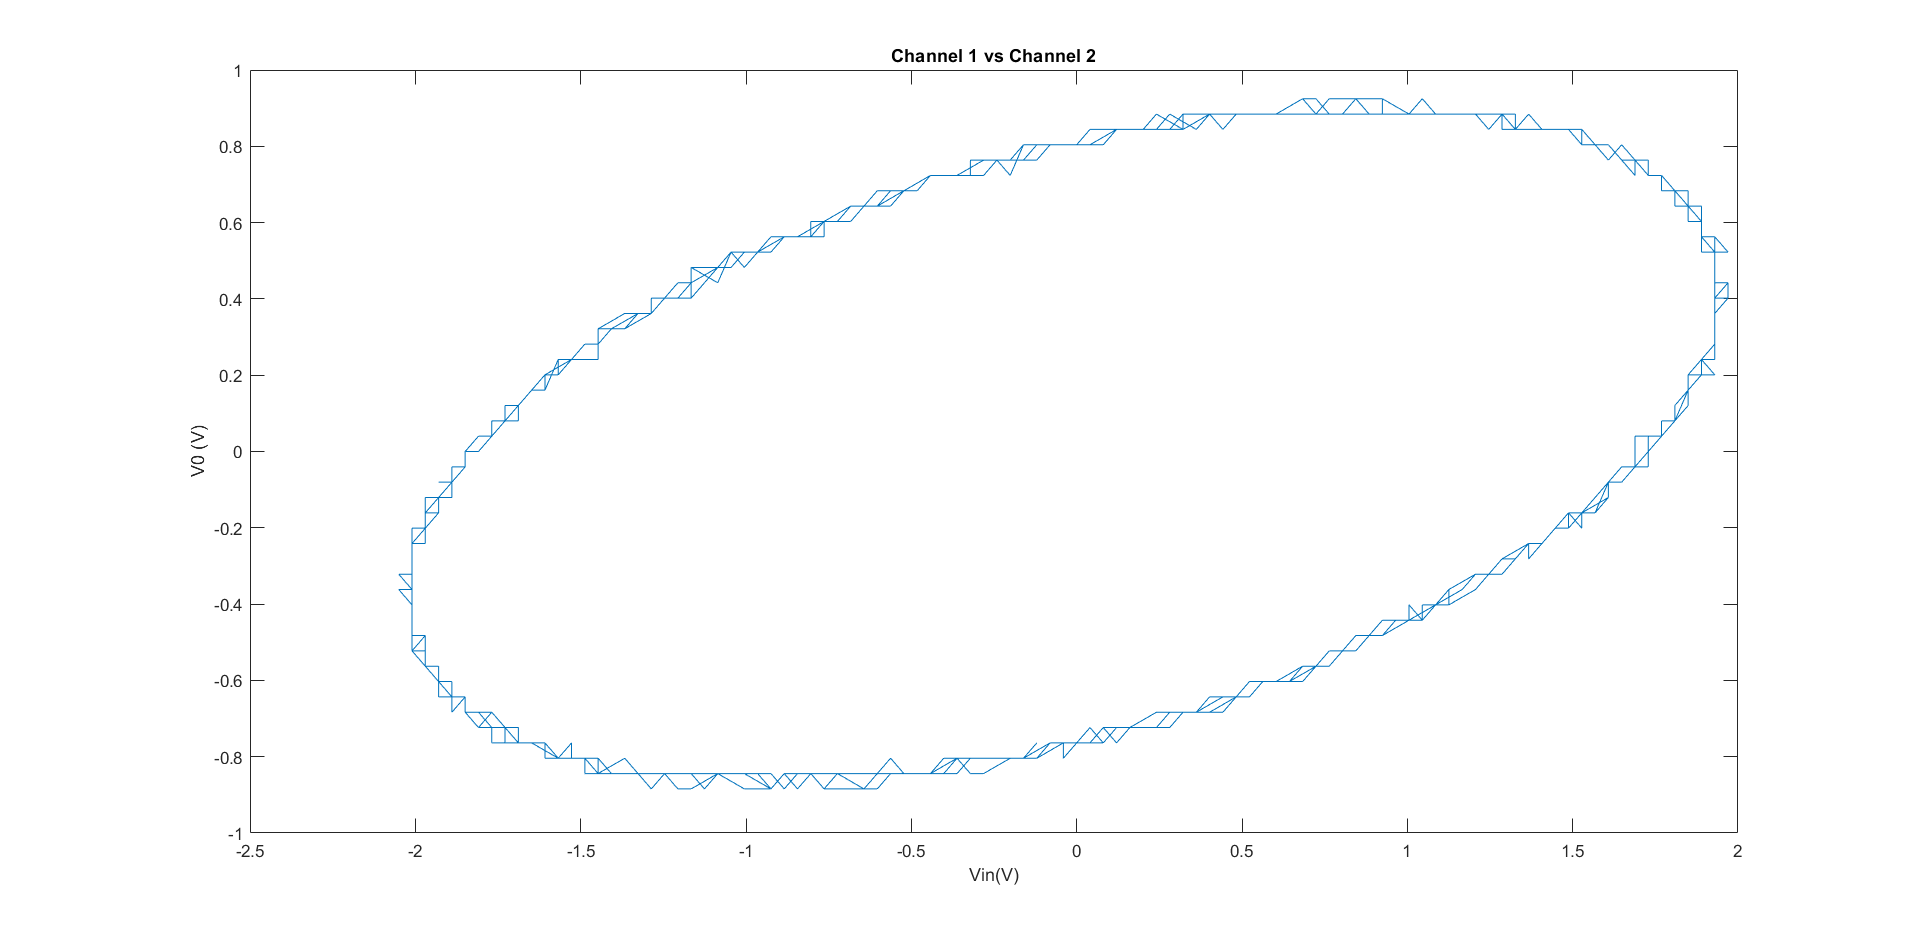
\includegraphics[width=1\textwidth]{6b.png}
\end{figure}

\subsection{Step 7}
The function waveform generator is adjusted 3 \(V_{pp}\) and frequency of 1.003 kHz. The "Channel 1" probes of the DSO is connected the generators' output after making sure that the "Channel 2" is deactivated. Using the measurement tools on the oscilloscope the properties of the autoscaled signal are measured. The  \(V_{pp}\) is displayed "3.06 Volts" . The period is displayed 998.8\( \mu \)s and the frequency is 1.003 kHz.


\subsection{Step 8}
In this step, in addition to the setup at Step 7 the "Channel 2" probes connected to the "Probe Comp" output and activated. Two waveforms observed on the screen.
\subsubsection{a.}
Using the trigger and source buttons on the oscilloscope, "CH 1" is selected as source. As a result while the "Channel 1" signal is steady the "Channel 2" signal became moving. 
\subsubsection{b.}
Using the trigger and source options on the oscilloscope, "CH 2" is selected as References. As a result while the "Channel 2" signal is steady the "Channel 1" signal became moving. 
\subsubsection{c.}
Small variations in the frequency of the output signal of the function generator is made. The signal slides are observed. To get two steady waveforms on the screen the frequency is adjusted to "1.001,170 kHz". The reason why there are slides when we adjust the frequency higher or lower can be stated that,  the reference time frame of the sliding signal does not fit with the reference time frame of the trigger source signal.

\subsection{Step 9}

\subsubsection{a.}

\subsubsection{b.}


\section{Conclusion}
The measurement features of the oscilloscope instrument is experienced.
\section{Appendix I}

%++++++++++++++++++++++++++++++++++++++++
% References section will be created automatically 
% with inclusion of "thebibliography" environment
% as it shown below. See text starting with line
% \begin{thebibliography}{99}
% Note: with this approach it is YOUR responsibility to put them in order
% of appearance.

\begin{thebibliography}{99}

%https://tr.overleaf.com/latex/templates/sample-lab-report-for-u-of-r-phys-349/pgsyqngcyjxk

\end{thebibliography}


\end{document}